\section{$t\bar{t}h$发现}
目前ATLAS实验搜寻$t\bar{t}h$通过以下衰变道进行:
\begin{itemize}
 \item $t\bar{t}(h\rightarrow b\bar{b})$
 \item $t\bar{t}(h\rightarrow \gamma\gamma)$
 \item $t\bar{t}h\rightarrow$ 多轻子\footnote{本文称tthML}
\end{itemize}
$t\bar{t}(h\rightarrow b\bar{b})$具有最大的衰变分支比,其主要信号特征是很高的$b$喷注数。$t\bar{t}(h\rightarrow \gamma\gamma)$虽然衰变分支比很小,
但得益于双光子的良好的分辨,这个分析道有很好的希格斯质量极点和信号纯度。
tthML并不显性关注某个中间过程,它根据轻子数或者$\tau_{had}$数分类,主要针对$h\rightarrow WW^*$, $h\rightarrow \tau\tau$和$h\rightarrow ZZ^*$\footnote{不包括$t\bar{t}h\rightarrow ZZ^*\rightarrow 4\ell$},相应的数图阶费曼图见\ref{fig:diagram_tthML_LO}。
这种搜寻策略是因为我们的目标是确定$t\bar{t}h$的产生率,而不是耦合常数测量。在\RunOne ATLAS和CMS已通过以上衰变道进行$t\bar{t}h$寻找\cite{Aad:2015iha,Aad:2015gra,Aad:2014lma,Khachatryan:2014qaa,Khachatryan:2015ila,Khachatryan:2016vau},
联合ATLAS和CMS结果(图\ref{fig:HiggsPromu_ATALS_CMS})给出信号强度$\mu_{t\bar{t}h}=\sigma/\sigma_{SM}=2.3^{+0.7}_{-0.6}$,超出主要来自tthML测量,其结果为$\mu_{t\bar{t}h}=2.1^{+1.4}_{-1.2}$,95\%置信度下上限为$\mu_{t\bar{t}h}<4.7$,对应观测(期望)显著性为1.8$\sigma$(0.9$\sigma$)。

13 TeV~$t\bar{t}h$总截面相比8 TeV结果增加了3.9倍\cite{Heinemeyer:2013tqa,XSWG13TeV},
并且随着更多数据的累积,$\mu_{t\bar{t}h}$测量精度会得到显著提升。2017年ATLAS利用\RunTwo 36.1 fb$^{-1}$数据报告了$t\bar{t}h$存在证据\cite{Aaboud:2017jvq},联合以上衰变道给出观测(期望)显著性为4.2$\sigma$(3.8$\sigma$),$\mu_{t\bar{t}h}$的最佳拟合值为$1.2\pm0.2(\text{stat})^{+0.3}_{-0.2}(\text{syst})$,与标准模型预期基本一致,值得指出的是,tthML最敏感,其观测(期望)显著性为4.1$\sigma$(2.8$\sigma$)。
2018年ATLAS与CMS联合\RunOne 和\RunTwo 部分数据分别宣告发现$t\bar{t}h$\cite{Aaboud:2018urx,PhysRevLett.120.231801},
相应的信号强度测量结果ATLAS为$\mu_{t\bar{t}h}=1.32\pm0.18(\text{stat})^{0.21}_{-0.19}(\text{syst})$,CMS为$\mu_{t\bar{t}h}=1.26^{+0.31}_{-0.26}$
,其中ATLAS tthML给出$\mu_{t\bar{t}h}=1.56^{+0.30}_{-0.29}(\text{stat})^{0.30}_{-0.27}(\text{syst})$。
本章将叙述利用\RunTwo 2015-2017年数据进行的tthML分析,
主要关注\ltwotau 衰变道,并分别给出\ltwotau 拟合结果和tthML联合拟合结果。
\begin{figure}[h]
\centering
 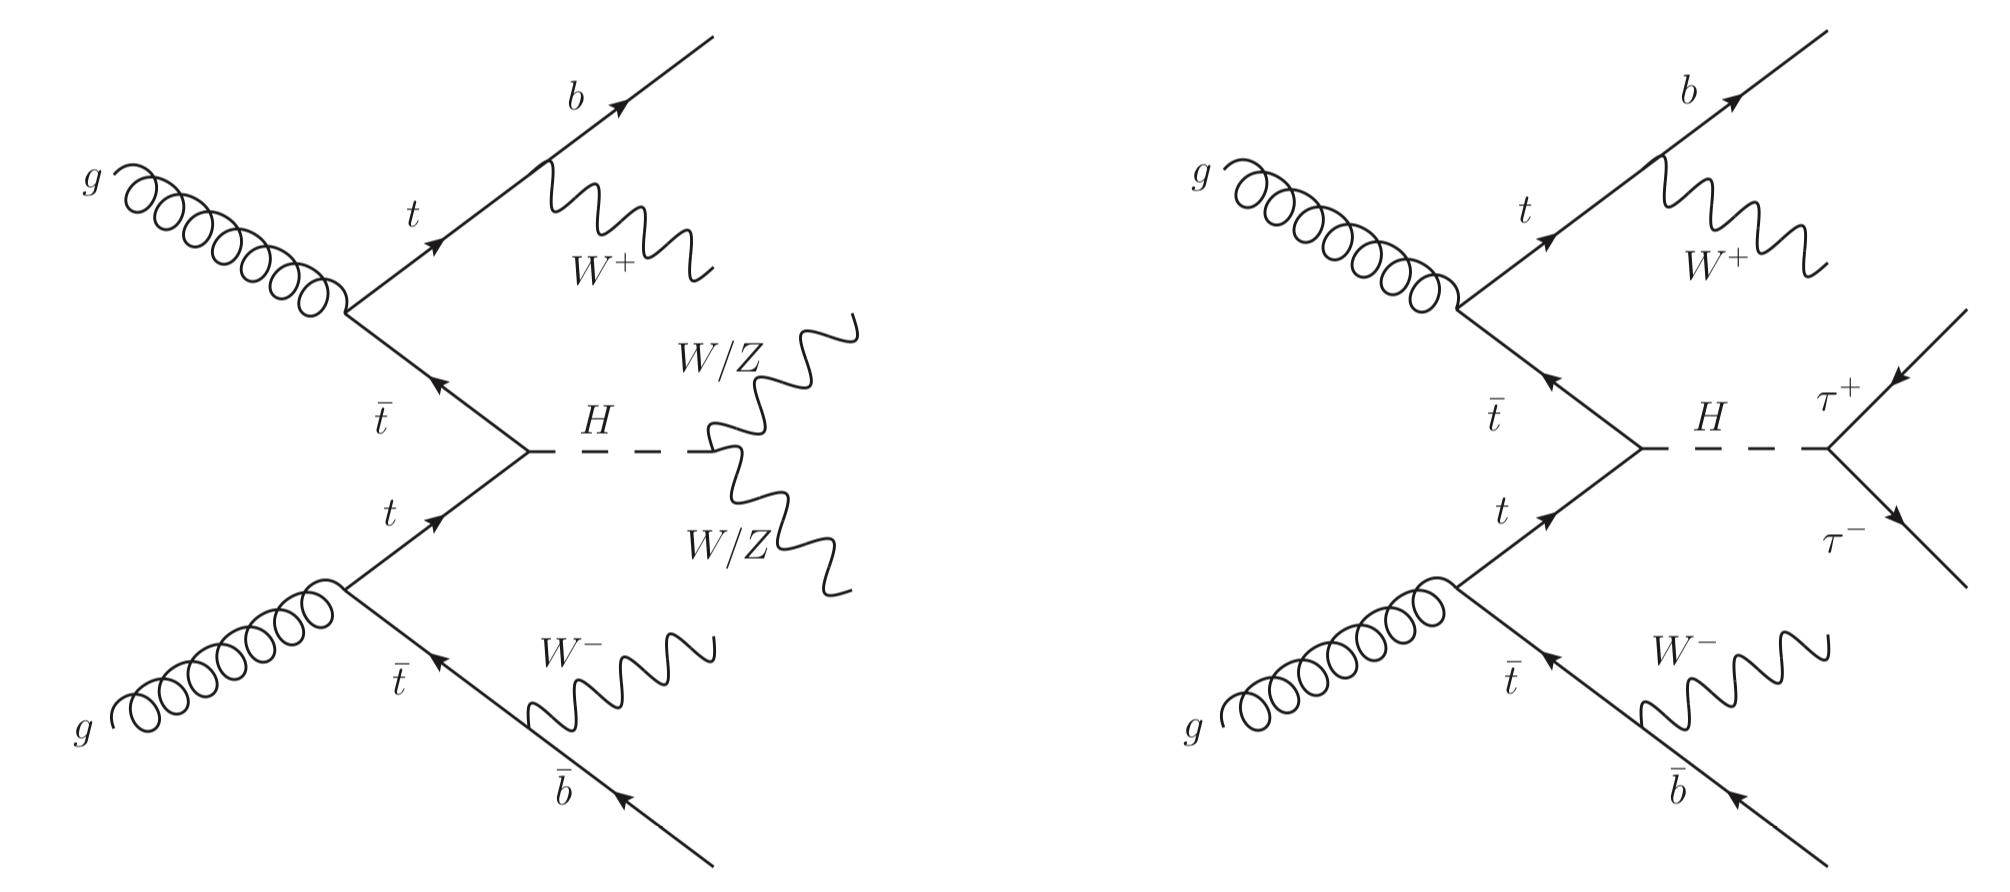
\includegraphics[width=0.7\textwidth]{fig/diagram_tth_LO.png}
 \caption{tthML树图阶费曼图,左图:$h\rightarrow WW^*/ZZ^*$,右图:$h\rightarrow \tau\tau$。}
 \label{fig:diagram_tthML_LO}
\end{figure}

\begin{figure}[h]
\centering
 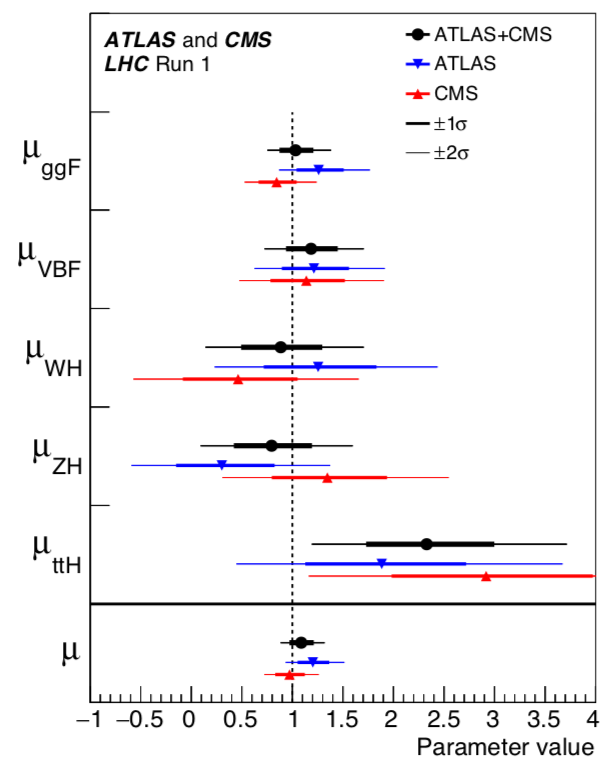
\includegraphics[width=0.7\textwidth]{fig/ATLAS_CMS_HiggsMes.png}
 \caption{Run 1联合ATLAS与CMS数据给出的希格斯产生模式最佳拟合值\cite{Khachatryan:2016vau},粗线表示1$\sigma$,细线表示2$\sigma$。}
 \label{fig:HiggsPromu_ATALS_CMS}
\end{figure}

\begin{figure}[h]
\centering
\begin{subfigure}[b]{0.95\textwidth}
\centering
 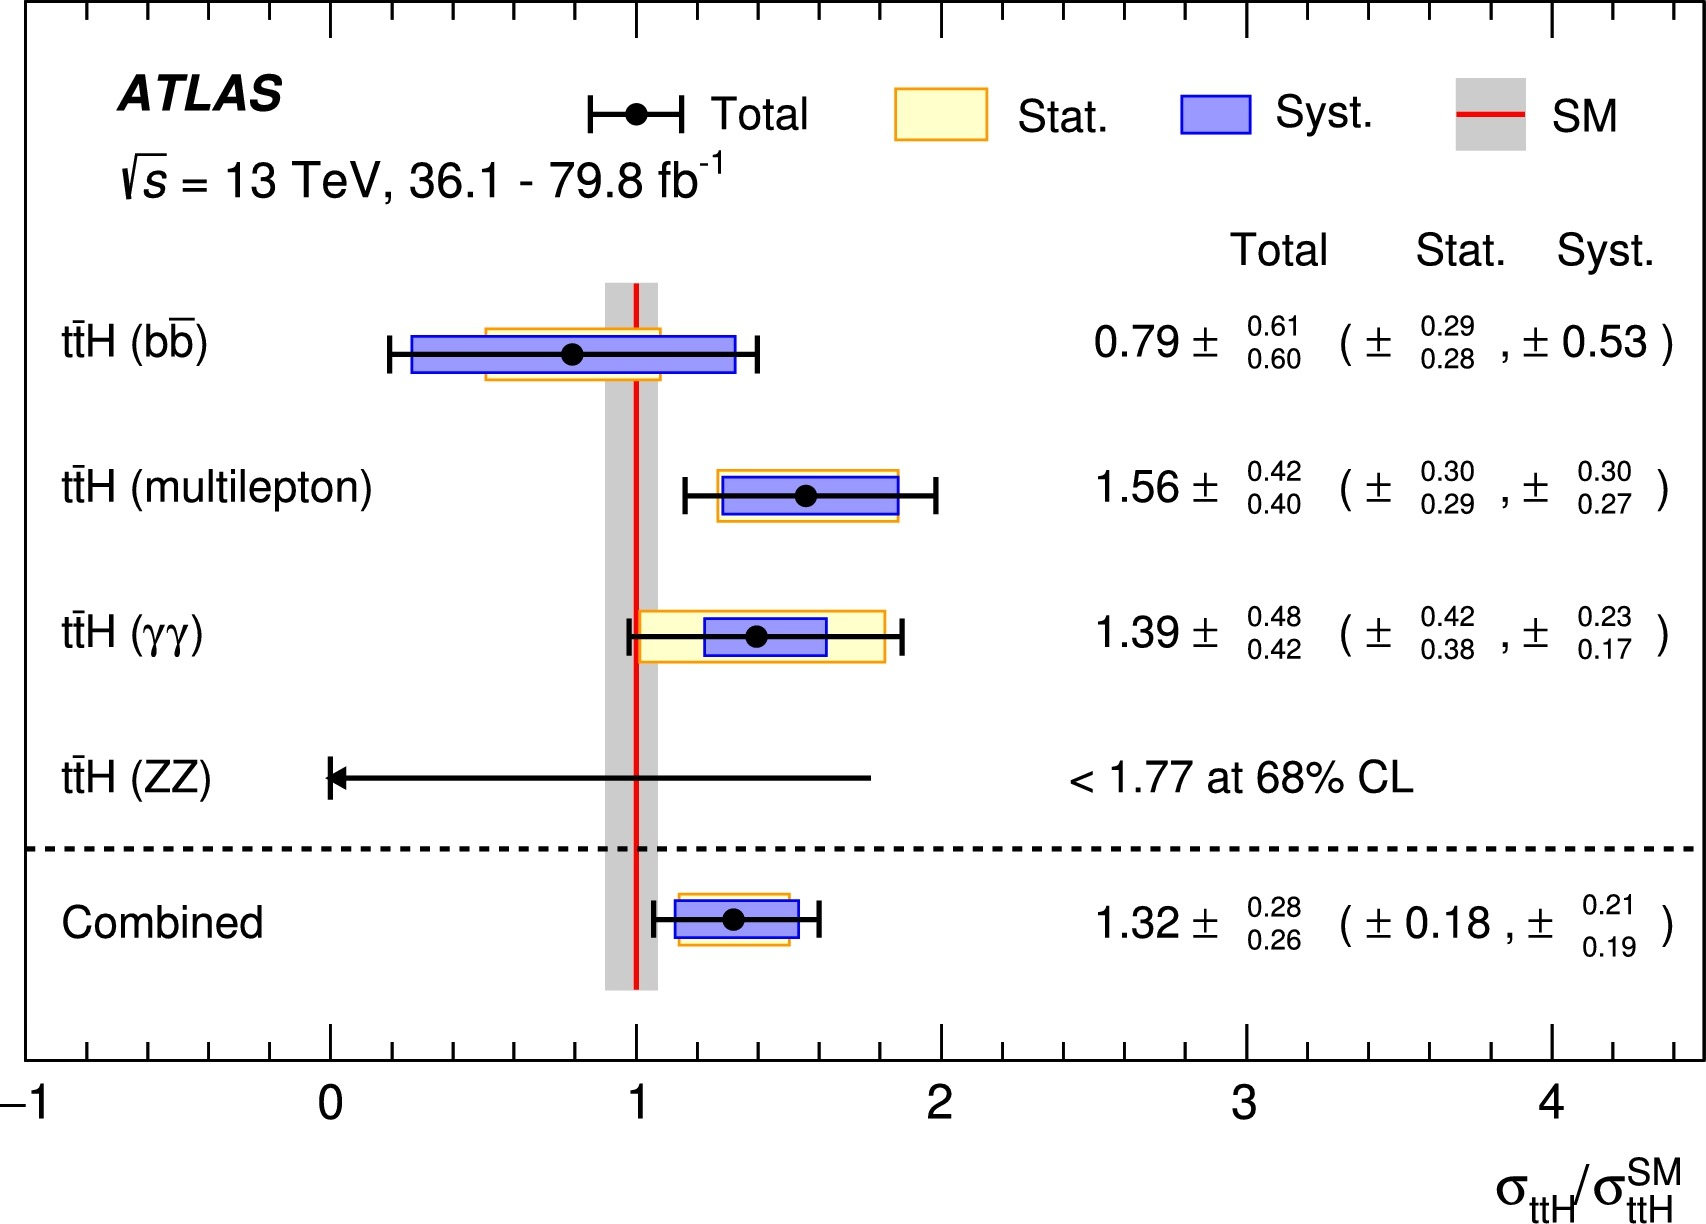
\includegraphics[width=0.75\textwidth]{fig/ATLAS_ttH_mu_80fb.jpg}
 \caption{ATLAS结果\cite{Aaboud:2018urx}}\label{subfig:ATLAS_tth_mu_80fb}
\end{subfigure}\\
\begin{subfigure}[b]{0.95\textwidth}
\centering
 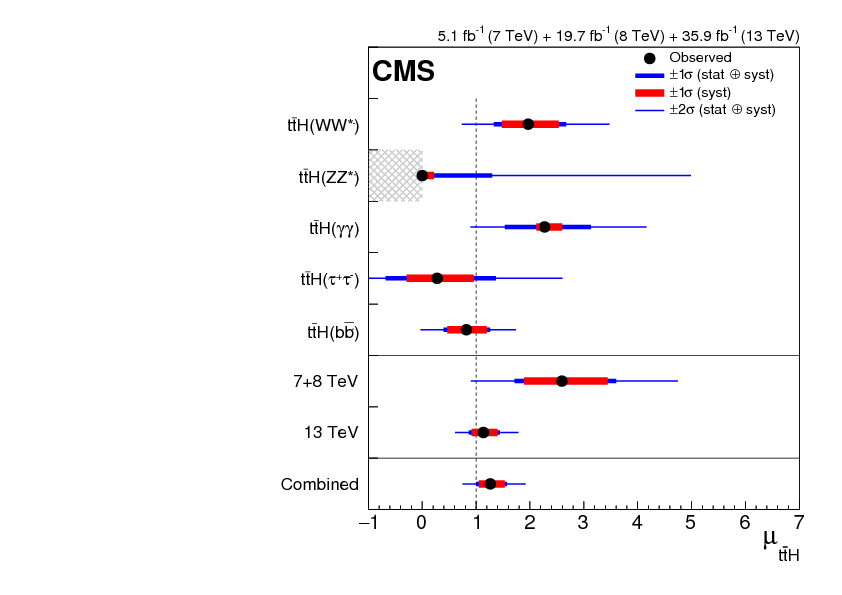
\includegraphics[width=0.75\textwidth]{fig/CMS_ttH_mu_80fb.png}
 \caption{CMS结果\cite{PhysRevLett.120.231801}}\label{subfig:CMS_tth_mu_80fb}
\end{subfigure}
 \caption{Run 2 $t\bar{t}h$信号强度测量结果。}
 \label{fig:HiggsPromu_ATALS_CMS}
\end{figure}

\section{tthML分类}
为了最大限度利用tthML数据,tthML会根据轻子数或者$\tau_{had}$数分类,最后联合拟合所有分析道得到信号强度。对于2015-2017年数据分析,tthML有以下六个分析道(图\ref{fig:tthML_cates}):
\begin{itemize}
 \item $2\ell\text{SS}$:两个相同电荷轻子,并且没有$\tau_{\text{had}}$。
 \item $3\ell$:三个轻子,总电荷为$\pm1$,并且没有$\tau_{\text{had}}$。
 \item $4\ell$:四个轻子,总电荷为0。
 \item $2\ell\text{SS}+1\tau_{\text{had}}$:两个相同电荷轻子,一个$\tau_{\text{had}}$。
% \item $2\ell\text{SS}+2\tau_{\text{had}}$:两个相同电荷轻子,两个$\tau_{\text{had}}$。
 \item $3\ell+1\tau_{\text{had}}$:三个轻子,总电荷为$\pm1$,一个$\tau_{\text{had}}$。
 \item \ltwotau :一个轻子,两个相反电荷的$\tau_{\text{had}}$。
\end{itemize}
%相应的分类也可见图\ref{fig:tthML_cates}
\begin{figure}[h]
\centering
 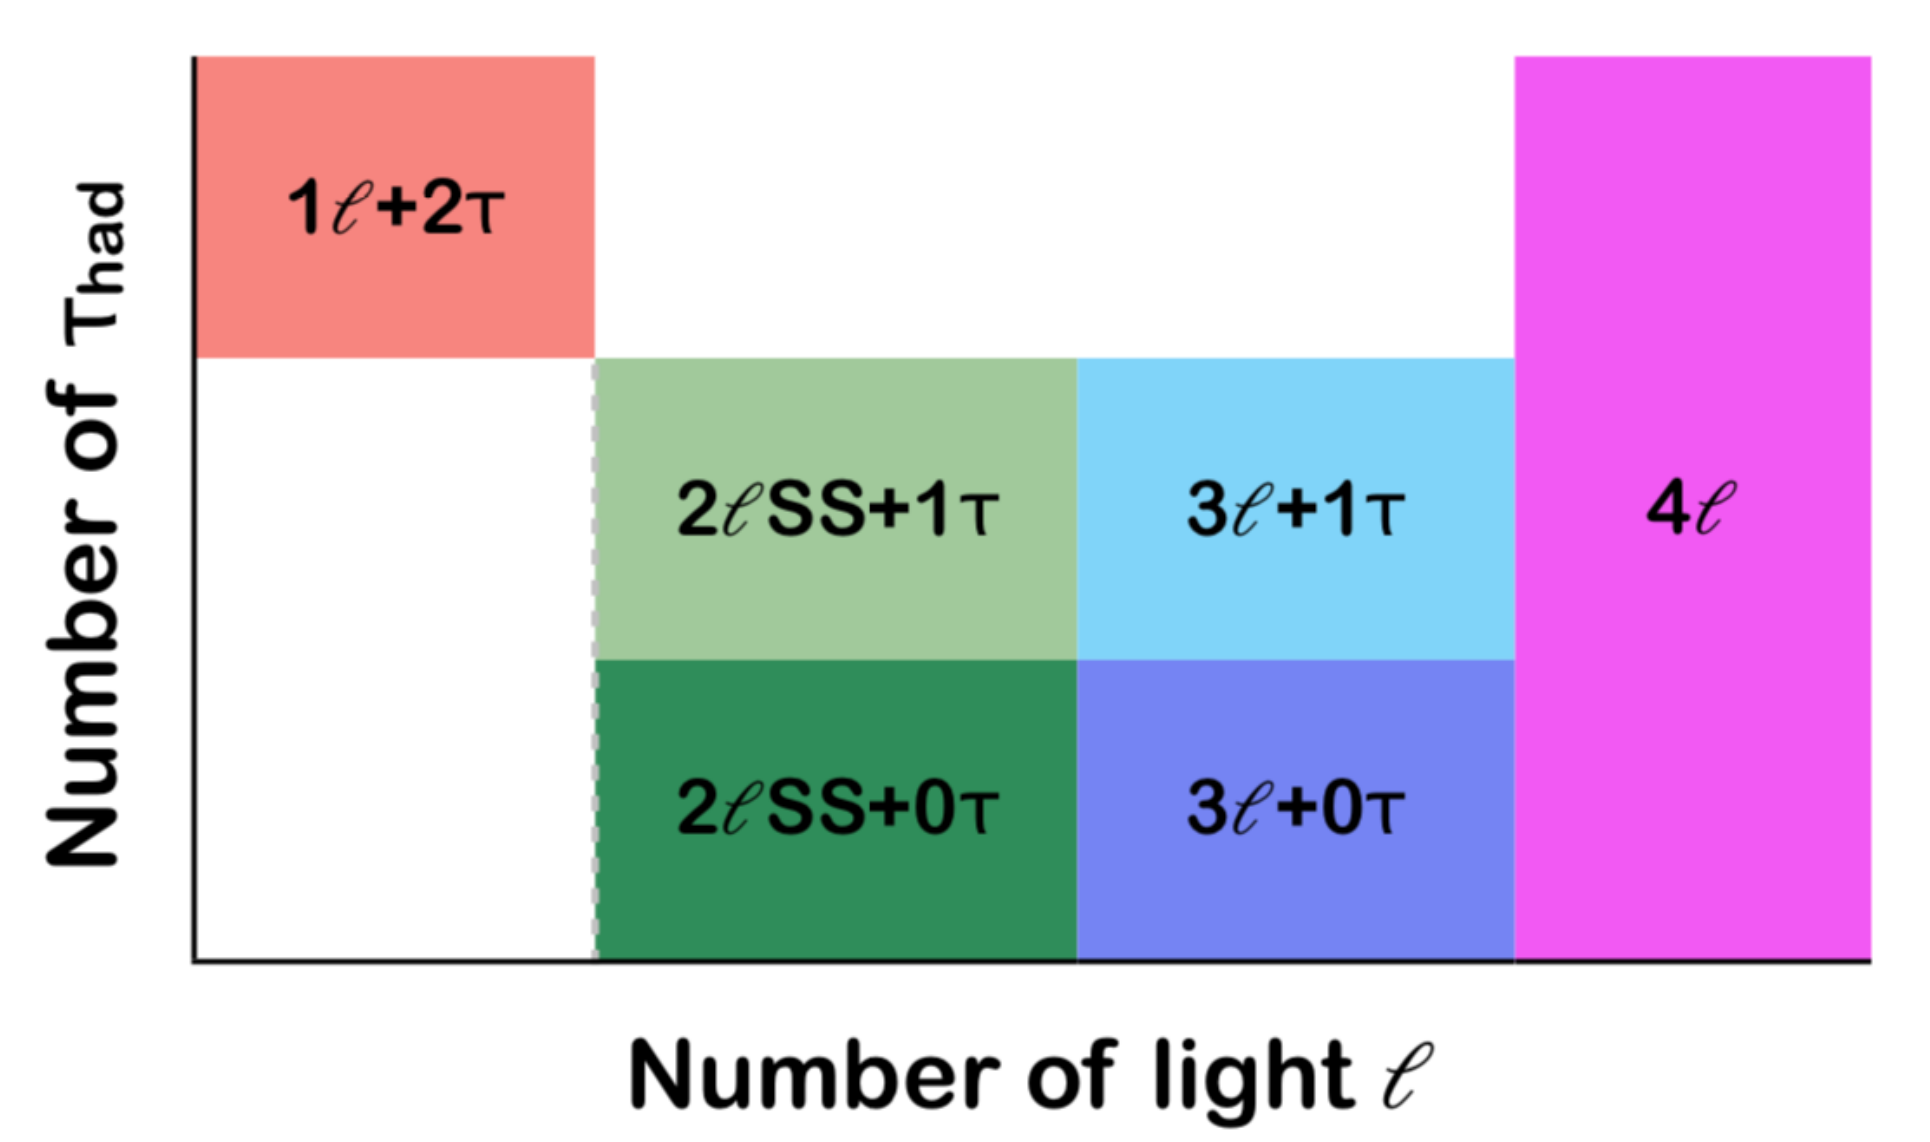
\includegraphics[width=0.75\textwidth]{fig/tthML_cates.png}
 \caption{tthML分类图示。}
 \label{fig:tthML_cates}
\end{figure}
如图\ref{fig:tthML_signal_comp}所示,不同类别对不同希格斯衰变敏感,$2\ell\text{SS}$,$3\ell$以及$4\ell$~的80\%信号来自$h\rightarrow WW^*$,并且$3\ell$和$4\ell$的一部分信号为$h\rightarrow ZZ^*$,大约为5\%$\sim$10\%,还观察到随着$\tau_{had}$数增加,$h\rightarrow \tau\tau$贡献越大,其中\ltwotau ~98\%信号贡献是$h\rightarrow \tau\tau$,这是
\ltwotau 的独特之处。另外,$4\ell$信号纯度($S/B$)最高,但是受限于统计量,显著性($S/\sqrt{B}$)一般,最高显著性为$2\ell\text{SS}$和$3\ell$。
\begin{figure}[h]
\centering
 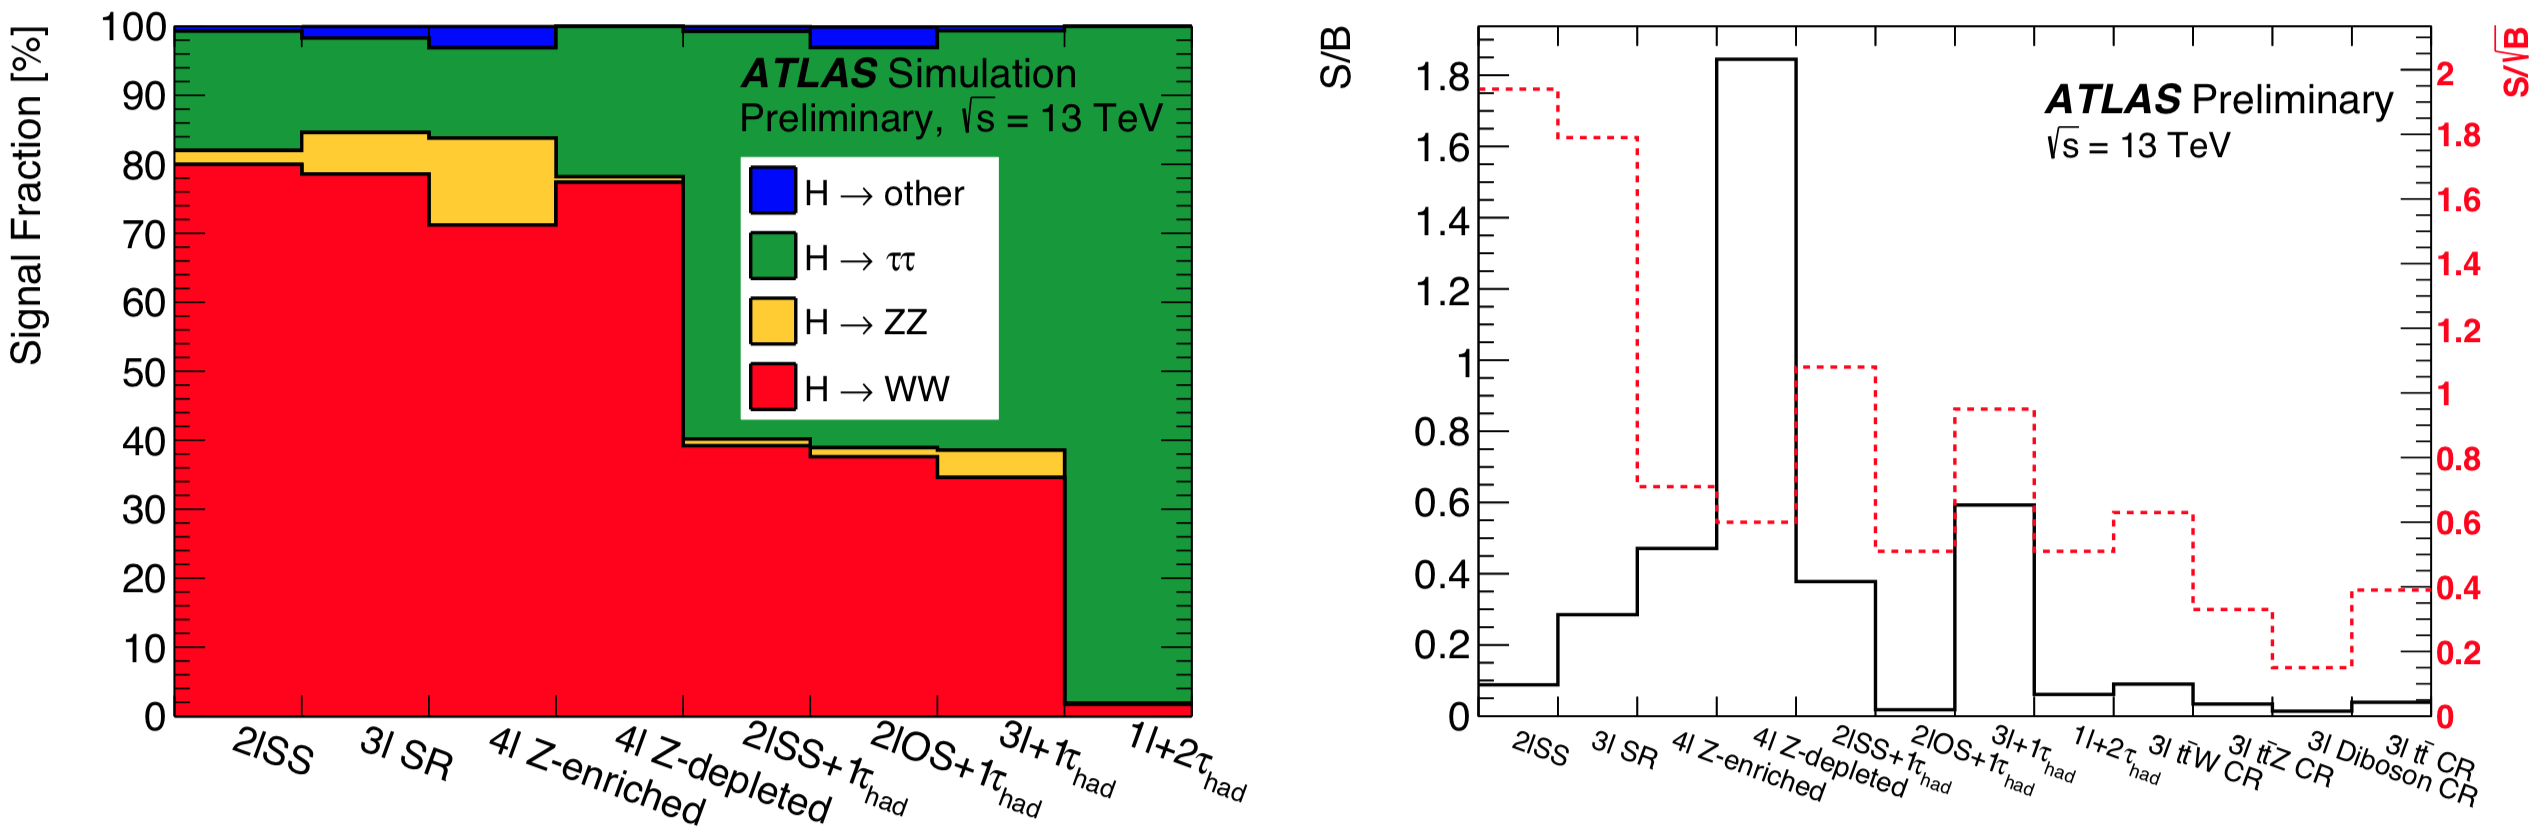
\includegraphics[width=0.85\textwidth]{fig/tthML_signal_comp.png}
 \caption{左图:tthML信号类别中希格斯衰变来源分布;右图:$S/B$(黑色),$S/\sqrt{B}$(红色)。其中'other'主要贡献来自$h\rightarrow \mu\mu$和$h\rightarrow b\bar{b}$。\cite{Aaboud:2017jvq}}
 \label{fig:tthML_signal_comp}
\end{figure}

\section{数据与MC}
本文tthML分析使用2015-2017年的对撞数据,总共80 fb$^{-1}$,具体收集情况可参见亮度章节\ref{fig:data_taking}。

表\ref{tab:mcconfig}总结信号与背景MC产生情况,所有希格斯粒子质量均设为125 GeV。\tth 通过\POWHEGBOX 产生,\ttz 通过\MGMCatNLO 在QCD次领头阶产生,两种样本而后
均使用\PYTHIA 8 模拟部分子簇射和强子化过程。单举\ttbar$\ell\ell$ 过程(包括\ttbar$\ell\ell$, \ttbar$\ell\ell+q/g$及\ttbar$\ell\ell+2q/g$)的硬散射模拟考虑了不在壳的$Z$玻色子和虚光子($\gamma^*$)贡献,要求$m(\ell\ell)>5$ GeV。$t\bar{t}W$ MC使用\textsc{Sherpa 2.2.5}产生,对于具有最多一个出射额外部分子事例在次领头阶计算,而对于其他事例在领头阶计算。
\tth 总截面为507.1 fb,在QCD次领头阶和使用电弱参数\cite{Beenakker:2001rj,Beenakker:2002nc,Dawson:2002tg,Dawson:2003zu,Yu:2014cka,Frixione:2014qaa,Frixione:2015zaa}计算得到\cite{Heinemeyer:2013tqa,XSWG13TeV},来自QCD重整化和因子化的误差为$^{+5.8\%}_{-9.2\%}$,来自PDF和$\alpha_s$的误差为$\pm3.6$\%。
$t\bar{t}V$(包括$pp\rightarrow t\bar{t}\ell^+\ell^-+X$)产生截面计算到QCD次领头阶\cite{Alwall:2014hca,Frixione:2015zaa},$\sigma_{t\bar{t}\ell\ell}$=123.7 fb,$\sigma_{t\bar{t}W}$=600.8 fb,它们的QCD scale误差大约12\%,PDF+$\alpha_s$误差为3-4\%。

\ttbar 事例使用\POWHEG v2.0和\PYTHIA 8仿真,其中\PYTHIA 8使用A14 tune。\ttbar 的产生截面832 pb。\POWHEG 也用于仿真其他单顶夸克过程,比如$Wt$。

$VV$(包括$VV+q/g$, $VV+2q/g$及$VV+3q/g$)事例使用\SHERPA v2.2.2仿真,其中对于$4\ell$, $3\ell+\nu$及$2\ell+2\nu$事例,如果最多有一个额外出射部分子,在次领头阶计算,
其他事例在领头阶计算。$W^{\pm}W^{\pm}jj$ MC分为QCD类($\mathcal{O}(\alpha_{em}^4\alpha_s^2)$)与VBS(Vector Boson Scattering)类($\mathcal{O}(\alpha_{em}^6)$),各自在领头阶产生\footnote{忽略相互干涉项}。额外的VBS过程,$qq\rightarrow3\ell\nu jj$, $qq\rightarrow 4\ell$和圈图过程$gg\rightarrow WZ^*/ZZ^*$也使用同样的方法产生。

最后如章节\ref{sec:evt_simulation}所述,所有的MC经过ATLAS探测器仿真,通过\PYTHIA 8产生的pileup事例\footnote{包括同时发生的$pp$对撞(in-time pileup)和附近不同时的pileup(out-of-time pileup)}也会叠加到一起。%而后所有MC如章节\ref{sec:evt_reco}所述一样进行事例重建。在tthML分析中,还会对粒子和事例进行进一步筛选,这会在随后章节叙述。

\begin{table}[h]
\begin{center}
{\small
\setlength\tabcolsep{1.5pt}
\scalebox{0.85}{
\begin{tabular}{llllll}
\hline\hline
Process & Generator & Parton Shower & PDF & Tune  \\
& (alternative) & (alternative) & & \\
\hline
$t\bar{t}h$ & \textsc{Powheg-BOX} \cite{powhegtt}  & \textsc{Pythia} 8\ & NNPDF 3.0 NLO \cite{Ball:2014uwa}/ & A14 \\
     &                                         &                                       & NNPDF 2.3 LO \cite{Ball:2012cx} \\
     & (-) & (\textsc{Herwig++}) &  \\
$thqb$ & \textsc{MG5\_aMC} & \textsc{Pythia} 8 & CT10 \cite{ct10} & A14  & \\
$thW$ & \textsc{MG5\_aMC} & \textsc{Herwig++}  & CT10 & UE-EE-5   \cite{Seymour:2013qka}   \\
& & & /CTEQ6L1 \cite{cteq6l1,cteq6}  \\
%$\ttbar W$ & \textsc{MG5\_aMC} & \textsc{Pythia} 8 & NNPDF 3.0 NLO & A14   \\
%& & & /2.3 LO \\
$t\bar{t}W$ & \textsc{Sherpa 2.2.5}~\cite{sherpa} & \textsc{Sherpa 2.2.5}  & NNPDF 3.0 NNLO  & \textsc{Sherpa} default   \\
& (\textsc{MG5\_aMC}) & (\textsc{Pythia} 8) &  \\
$t\bar{t} (Z/\gamma^*)$ & \textsc{MG5\_aMC} & \textsc{Pythia} 8 & NNPDF 3.0 NLO & A14  \\
&&& /2.3 LO \\
& (\textsc{Sherpa}) & (\textsc{Sherpa}) &  \\
$t (Z/\gamma^*)$ & \textsc{MG5\_aMC} & \textsc{Pythia} 8  & CTEQ6L1 & Perugia2012 \cite{perugia}  \\
$t W (Z/\gamma^*)$ & \textsc{MG5\_aMC} & \textsc{Pythia} 8 & NNPDF 2.3 LO  & A14  \\
$t\bar t t$, $t\bar t t\bar t$ & \textsc{MG5\_aMC} & \textsc{Pythia} 8 & NNPDF 2.3 LO & A14 \\
$t\bar t W^+ W^-$ & \textsc{MG5\_aMC} & \textsc{Pythia} 8 & NNPDF 2.3 LO & A14  \\
$t\bar{t}$ & \textsc{Powheg-BOX} \cite{powhegtt} & \textsc{Pythia} 8 & CT10/CTEQ6L1 & Perugia2012  \\
$t\bar{t}\gamma$ & \textsc{MG5\_aMC} & \textsc{Pythia} 8 & NNPDF 2.3 LO & A14  \\
$s$-, $t$-channel, & \textsc{Powheg-BOX} \cite{powhegstp,powhegstp2} & \textsc{Pythia} 6 & CT10 & Perugia2012   \\
 $Wt$ single top & & & /CTEQ6L1 \\
$VV$, $qqVV$, & \textsc{Sherpa} 2.2.2 \cite{sherpa} & \textsc{Sherpa} & NNPDF 3.0 NNLO & \textsc{Sherpa} default  \\
$VVV$ & & & \\
$Z \to \ell^+\ell^-$ & \textsc{Sherpa} 2.2 & \textsc{Sherpa} & NNPDF 3.0 NLO & \textsc{Sherpa} default \\
%$W \to \ell\nu$ & \textsc{Sherpa} & \textsc{Sherpa} & CT10 & \textsc{Sherpa} default \\
\hline\hline
\end{tabular}}
}
\caption{\label{tab:mcconfig} 
信号与背景MC产生子总结。对每一项过程,如果表中只有一个PDF,则表示硬散射和部分子簇射过程使用相同的PDF;如果有两个PDF,则前者用于硬散射,后者用于部分子簇射。
$V$指代$W$或者$Z/\gamma^*$。Tune指代部分子簇射产生子使用的次级碰撞微调器(underlying-event tune)。\textsc{MG5\_aMC}是\textsc{MadGraph5\_aMC@NLO} 2.2.1~\cite{Alwall:2014hca},
\textsc{Pythia} 6指代版本6.427~\cite{pythia6},\textsc{Pythia} 8指代版本8.2~\cite{pythia8},\textsc{Herwig++}指代版本2.7~\cite{Bahr:2008pv}。通过\PYTHIA 6或者\PYTHIA 8产生的MC使用\textsc{EvtGen} 1.2.0~\cite{Lange:2001uf}模拟,所有MC均考虑领头阶对数光子辐射(leading-logarithm photon emission),这通过部分子簇射产生子或者\textsc{PHOTOS}~\cite{Golonka:2005pn}仿真。
}
%The configurations used for event generation of signal and background processes.
%If only one parton distribution function (PDF) is shown, the same one is used for both the matrix element (ME) and parton shower generators;
%if two are shown, the first is used for the matrix element calculation and the second for the parton shower.  ``V'' refers to production of
%an electroweak boson ($W$ or $Z/\gamma^*$).  ``Tune'' refers to the underlying-event tune of the parton shower generator. ``\textsc{MG5\_aMC}''
%refers to \textsc{MadGraph5\_aMC@NLO} 2.2.1~\cite{Alwall:2014hca}; ``\textsc{Pythia} 6'' refers to version 6.427~\cite{pythia6}; ``\textsc{Pythia} 8''
%refers to version 8.2~\cite{pythia8}; ``\textsc{Herwig++}'' refers to version 2.7~\cite{Bahr:2008pv}.  Samples using \textsc{Pythia} 6 or \textsc{Pythia} 8
%have heavy flavour hadron decays modelled by \textsc{EvtGen} 1.2.0~\cite{Lange:2001uf}.  All samples include leading-logarithm photon emission, either modelled
%by the parton shower generator or by \textsc{PHOTOS}~\cite{Golonka:2005pn}.}
\end{center}
\end{table}

\section{粒子定义}\label{sec:obj_tth}
粒子重建及鉴别遵循章节\ref{sec:evt_reco}所述的一般方法。不同研究组对一般方法得到的重建粒子会进行适用于实际分析的筛选,称为粒子定义。出于本底研究,信号优化,假粒子压低等等目的,一般粒子会有两套甚至多套定义,不同定义之间可以互斥,可以相交。比如可定义筛选条件较松的Loose粒子,用于事例初步筛选或者本底研究,在Loose基础上定义Tight粒子,用于最终的信号区。本文将在随后的分析中涉及到此类定义。
tthML对不同粒子有(多套)不同定义,下面小节记录主要用于\ltwotau 分析的基本粒子筛选条件。

电子要求$\pt >$ 10 GeV,$\abseta <$2.47~(排除电磁量能器过渡区),\texttt{LooseLH} ID,横向径迹参数显著性(trasverse impact parameter significance)$|d_0|/\sigma_{d0}<$5,轴向径迹参数(longitudinal impact parameter)$|z_0sin\theta|<$0.5 mm。$\mu$子要求$\pt >$ 10 GeV,$\abseta <$2.5,\texttt{Loose} ID,$|d_0|/\sigma_{d0}<$3,$|z_0sin\theta|<$0.5 mm。值得一提的是,tthML分析大量使用了利用多变量方法开发的压低来自重味强子衰变轻子的变量(\texttt{PromptLeptonVeto})和压低电子电荷误判的变量(\texttt{ElectronChargeIDSelectionTool})\footnote{因为\ltwotau 轻子纯度较高,并未使用这两个变量。}。

$\tau_{\text{had}}$要求$\pt >$25 GeV, $\abseta <$2.5~(排除电磁量能器过渡区)。基于量能器和径迹信息训练的BDT变量用于鉴别真实$\tau_{\text{had}}$和压低喷注本底。所选的工作点对one-(three-)prong $\tau_{\text{had}}$有75\% (59\%)的选择效率\footnote{对应\texttt{medium} $\tau_{\text{had}}$ ID working point.}。BDT方法也用于排除被误判成one-prong $\tau_{\text{had}}$的电子
,该方法基于$Z\rightarrow ee$事例(重建后含有一个电子和一个$\tau_{\text{had}}$)训练,分析中使用的工作点对于真实$\tau_{\text{had}}$选择效率为95\%,对应的排除因子(rejection factor)依赖$\eta$与\pt ,大约在30到100。源自$\mu$子误判的$\tau_{\text{had}}$如果与$\mu$子($\pt >$2 GeV)距离很近,并且$\mu$子没有在量能器沉积能量(Calo-tagged),则丢掉$\tau_{\text{had}}$。
$\tau_{\text{had}}$也可能源自$b$喷注,与$\mu$子误判类似,如果$\tau_{\text{had}}$与$b$喷注(70\% WP)距离很近,则丢掉$\tau_{\text{had}}$。最后,为了压低pileup喷注的影响,$\tau_{\text{had}}$要求匹配初始顶点。

喷注筛选基本与章节\ref{subsec:jet_reco}所述一致。分析使用的喷注要求$\abseta <$2.5,而压低pileup喷注的JVT条件仅针对$\abseta <$2.4,所以在$2.4<\abseta <2.5$区间内软喷注仍可以来自
pileup。图\ref{fig:jet:jvteta}检查了数据,信号MC,$t\bar{t}$ MC中的喷注随\abseta 分布,可以看到在$2.4<\abseta <2.5$区间内并未看到明显喷注数增长,所以可以排除以上担忧。
\begin{figure}[h]
\centering
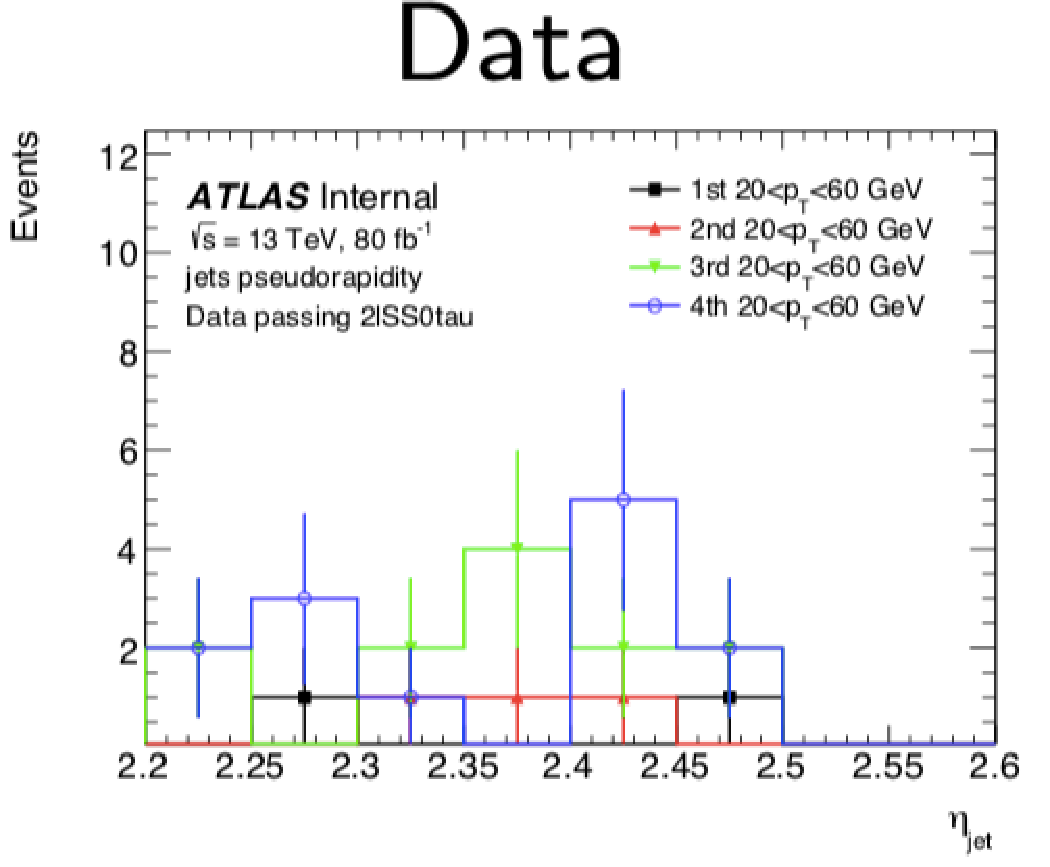
\includegraphics[width=0.3\textwidth]{fig/JVTData.pdf}
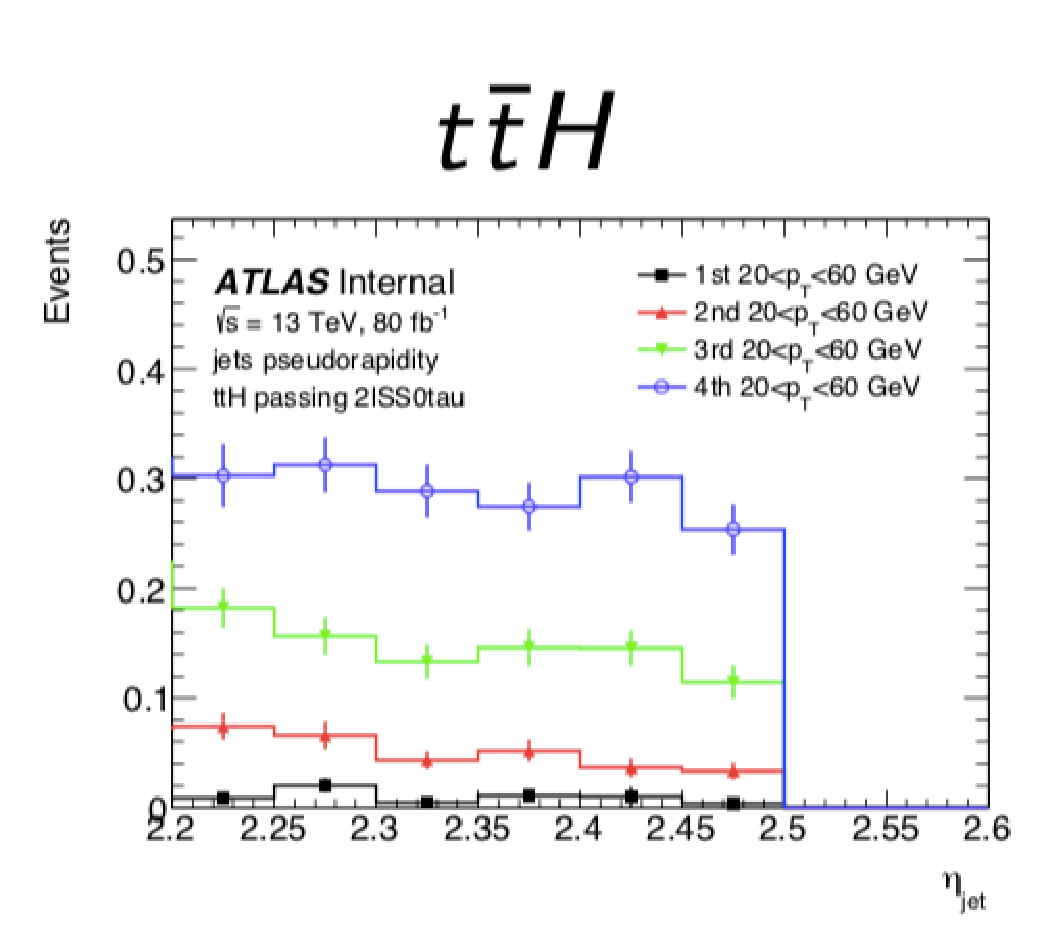
\includegraphics[width=0.3\textwidth]{fig/JVTttH.pdf}
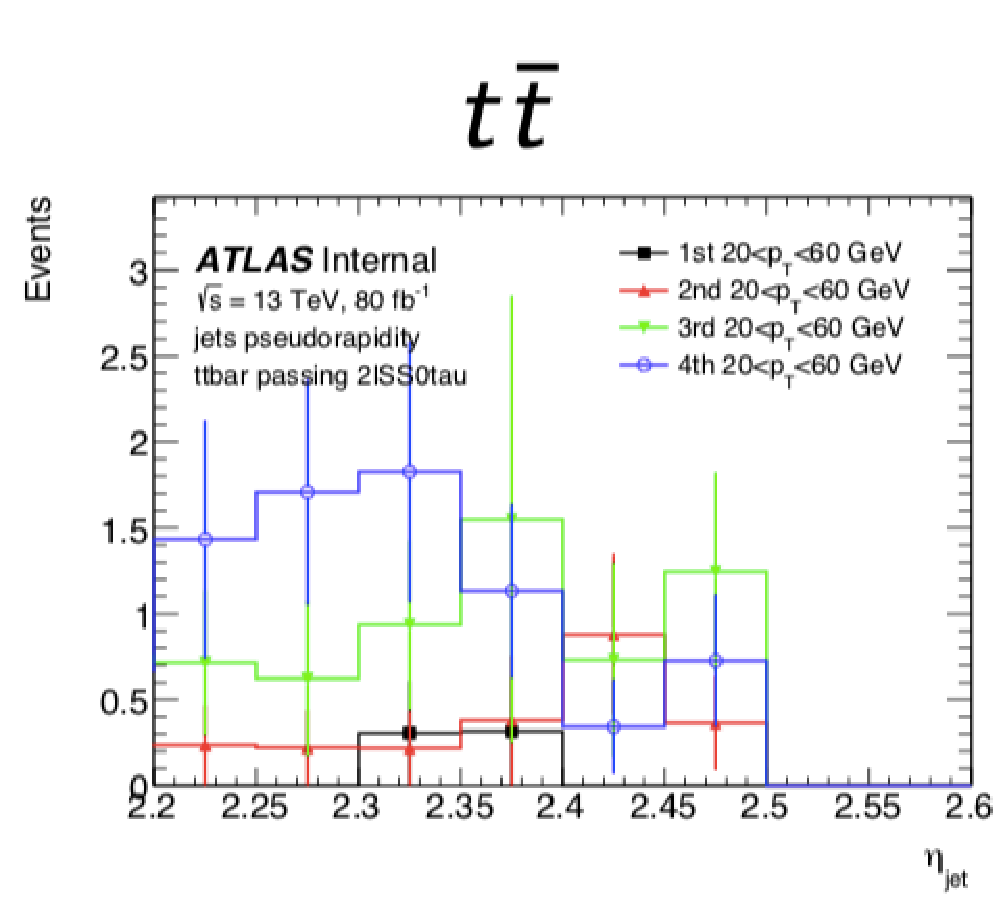
\includegraphics[width=0.3\textwidth]{fig/JVTttbar.pdf}
\caption{喷注随\abseta 分布,所选事例通过$2\ell\text{SS}$初步筛选,喷注按照\pt 排序,所以领头喷注的总事例数最少。总体上,分布没有明显的\abseta 依赖,可以排除由于JVT造成的影响。}
%\caption{Stability of jet yields as a function of $|\eta|$ threshold used for JVT for data (left), signal (middle) and $t\bar{t}$(right). No significant dependence is observed.  
\label{fig:jet:jvteta}
\end{figure}

$b$喷注定义与章节\ref{subsec:jet_reco}所述一致,使用70\% WP。

\met 定义遵循章节\ref{subsec:met_reco}所述,TST项使用径迹探测器信息。

\section{重叠移除}
不同的粒子流算法利用不同的输入有可能把实际上一个对象最终重建成相距很近的两个不同对象,
比如强子衰变出射一个轻子,重建之后得到一个喷注和一个轻子。为了避免此类重复计数问题,需要进行相应的重叠移除(overlap removal)\cite{Adams:1743654},
其方法就是移除相距较近粒子的其中一个。tthML的具体移除顺序可见表\ref{tab:overlap-removal-tth},不再赘述,需要注意的是所有粒子应当已通过章节\ref{sec:obj_tth}所述的基本定义条件。
\begin{table}[h]
 \begin{center}
   \begin{tabular}{c|c|c}
     \hline
                            \bf{Keep}  &  \bf{Remove} & \bf{Cone size ($\Delta$ R)}  \\
         \hline
                        electron        & electron (low \pt)    & 0.1 \\
     \hline
                        muon    & electron      & 0.1 \\
     \hline
                            electron    & jet   & 0.3 \\
         \hline
                        jet             & muon  & min(0.4, $0.04+10$[GeV]/\pt(muon)) \\
         \hline
                        electron        & tau   & 0.2 \\
     \hline
                        muon    & tau   & 0.2 \\
     \hline
                        tau             & jet   & 0.3 \\
     \hline
   \end{tabular}
   \caption{\label{tab:overlap-removal-tth}tthML 重叠移除总结,移除顺序从上到下。}
   %Summary of the overlap removal procedure between electrons, muons, hadronically decaying taus, and jets.}
 \end{center}
\end{table}
